\appendix{Представление графического материала}

Графический материал, выполненный на отдельных листах,
изображен на рисунках А.1--А.\arabic{числоПлакатов}.
\setcounter{числоПлакатов}{0}

\renewcommand{\thefigure}{А.\arabic{figure}} % шаблон номера для плакатов

\begin{landscape}

\begin{плакат}
    
\includegraphics[width=0.82\linewidth]{плакатТитульный.eps}
    \заголовок{Сведения о ВКРБ}
    \label{pl1:плакатТитульный}      
\end{плакат}

\begin{плакат}
	
\includegraphics[width=0.82\linewidth]{плакатЦельИЗадачи.eps}
	\заголовок{Цель и задачи разработки}
	\label{pl2:плакатЦельИЗадачи}      
\end{плакат}

\begin{плакат}
	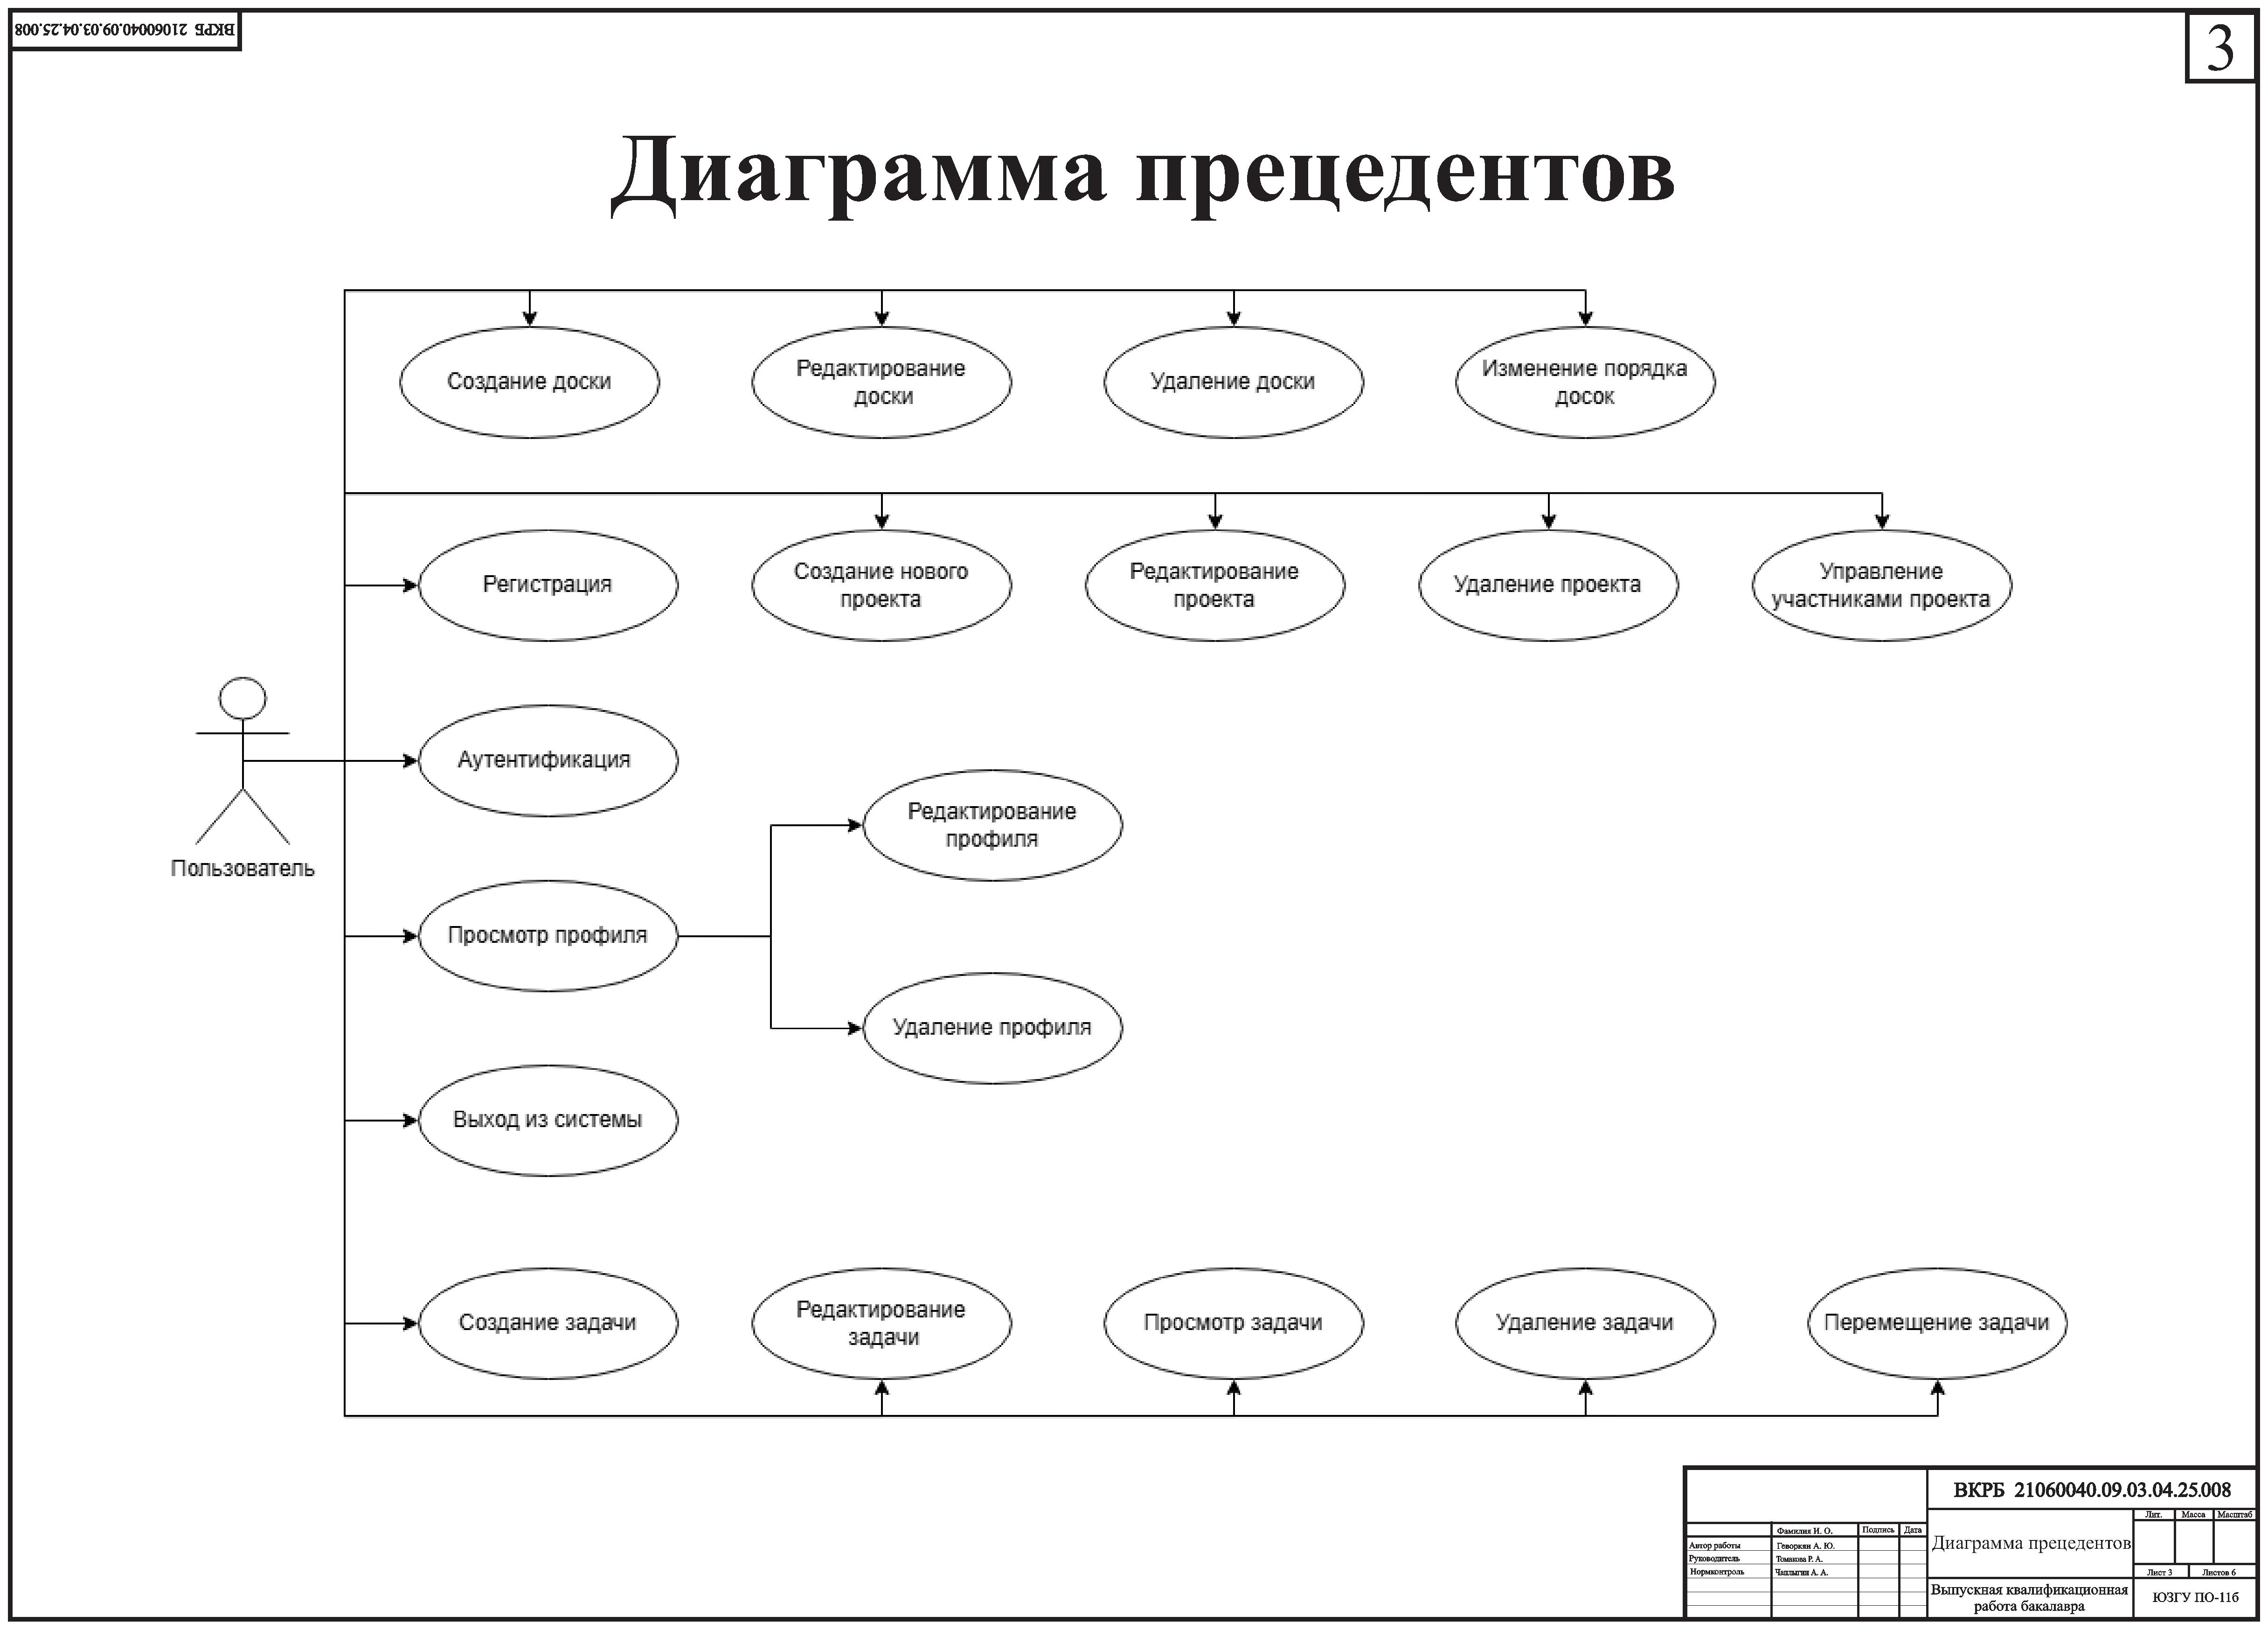
\includegraphics[width=0.82\linewidth]{плакатПрецеденты.eps}
	\заголовок{Диаграмма прецедентов}
	\label{pl3:плакатПрецеденты}      
\end{плакат}

\begin{плакат}
	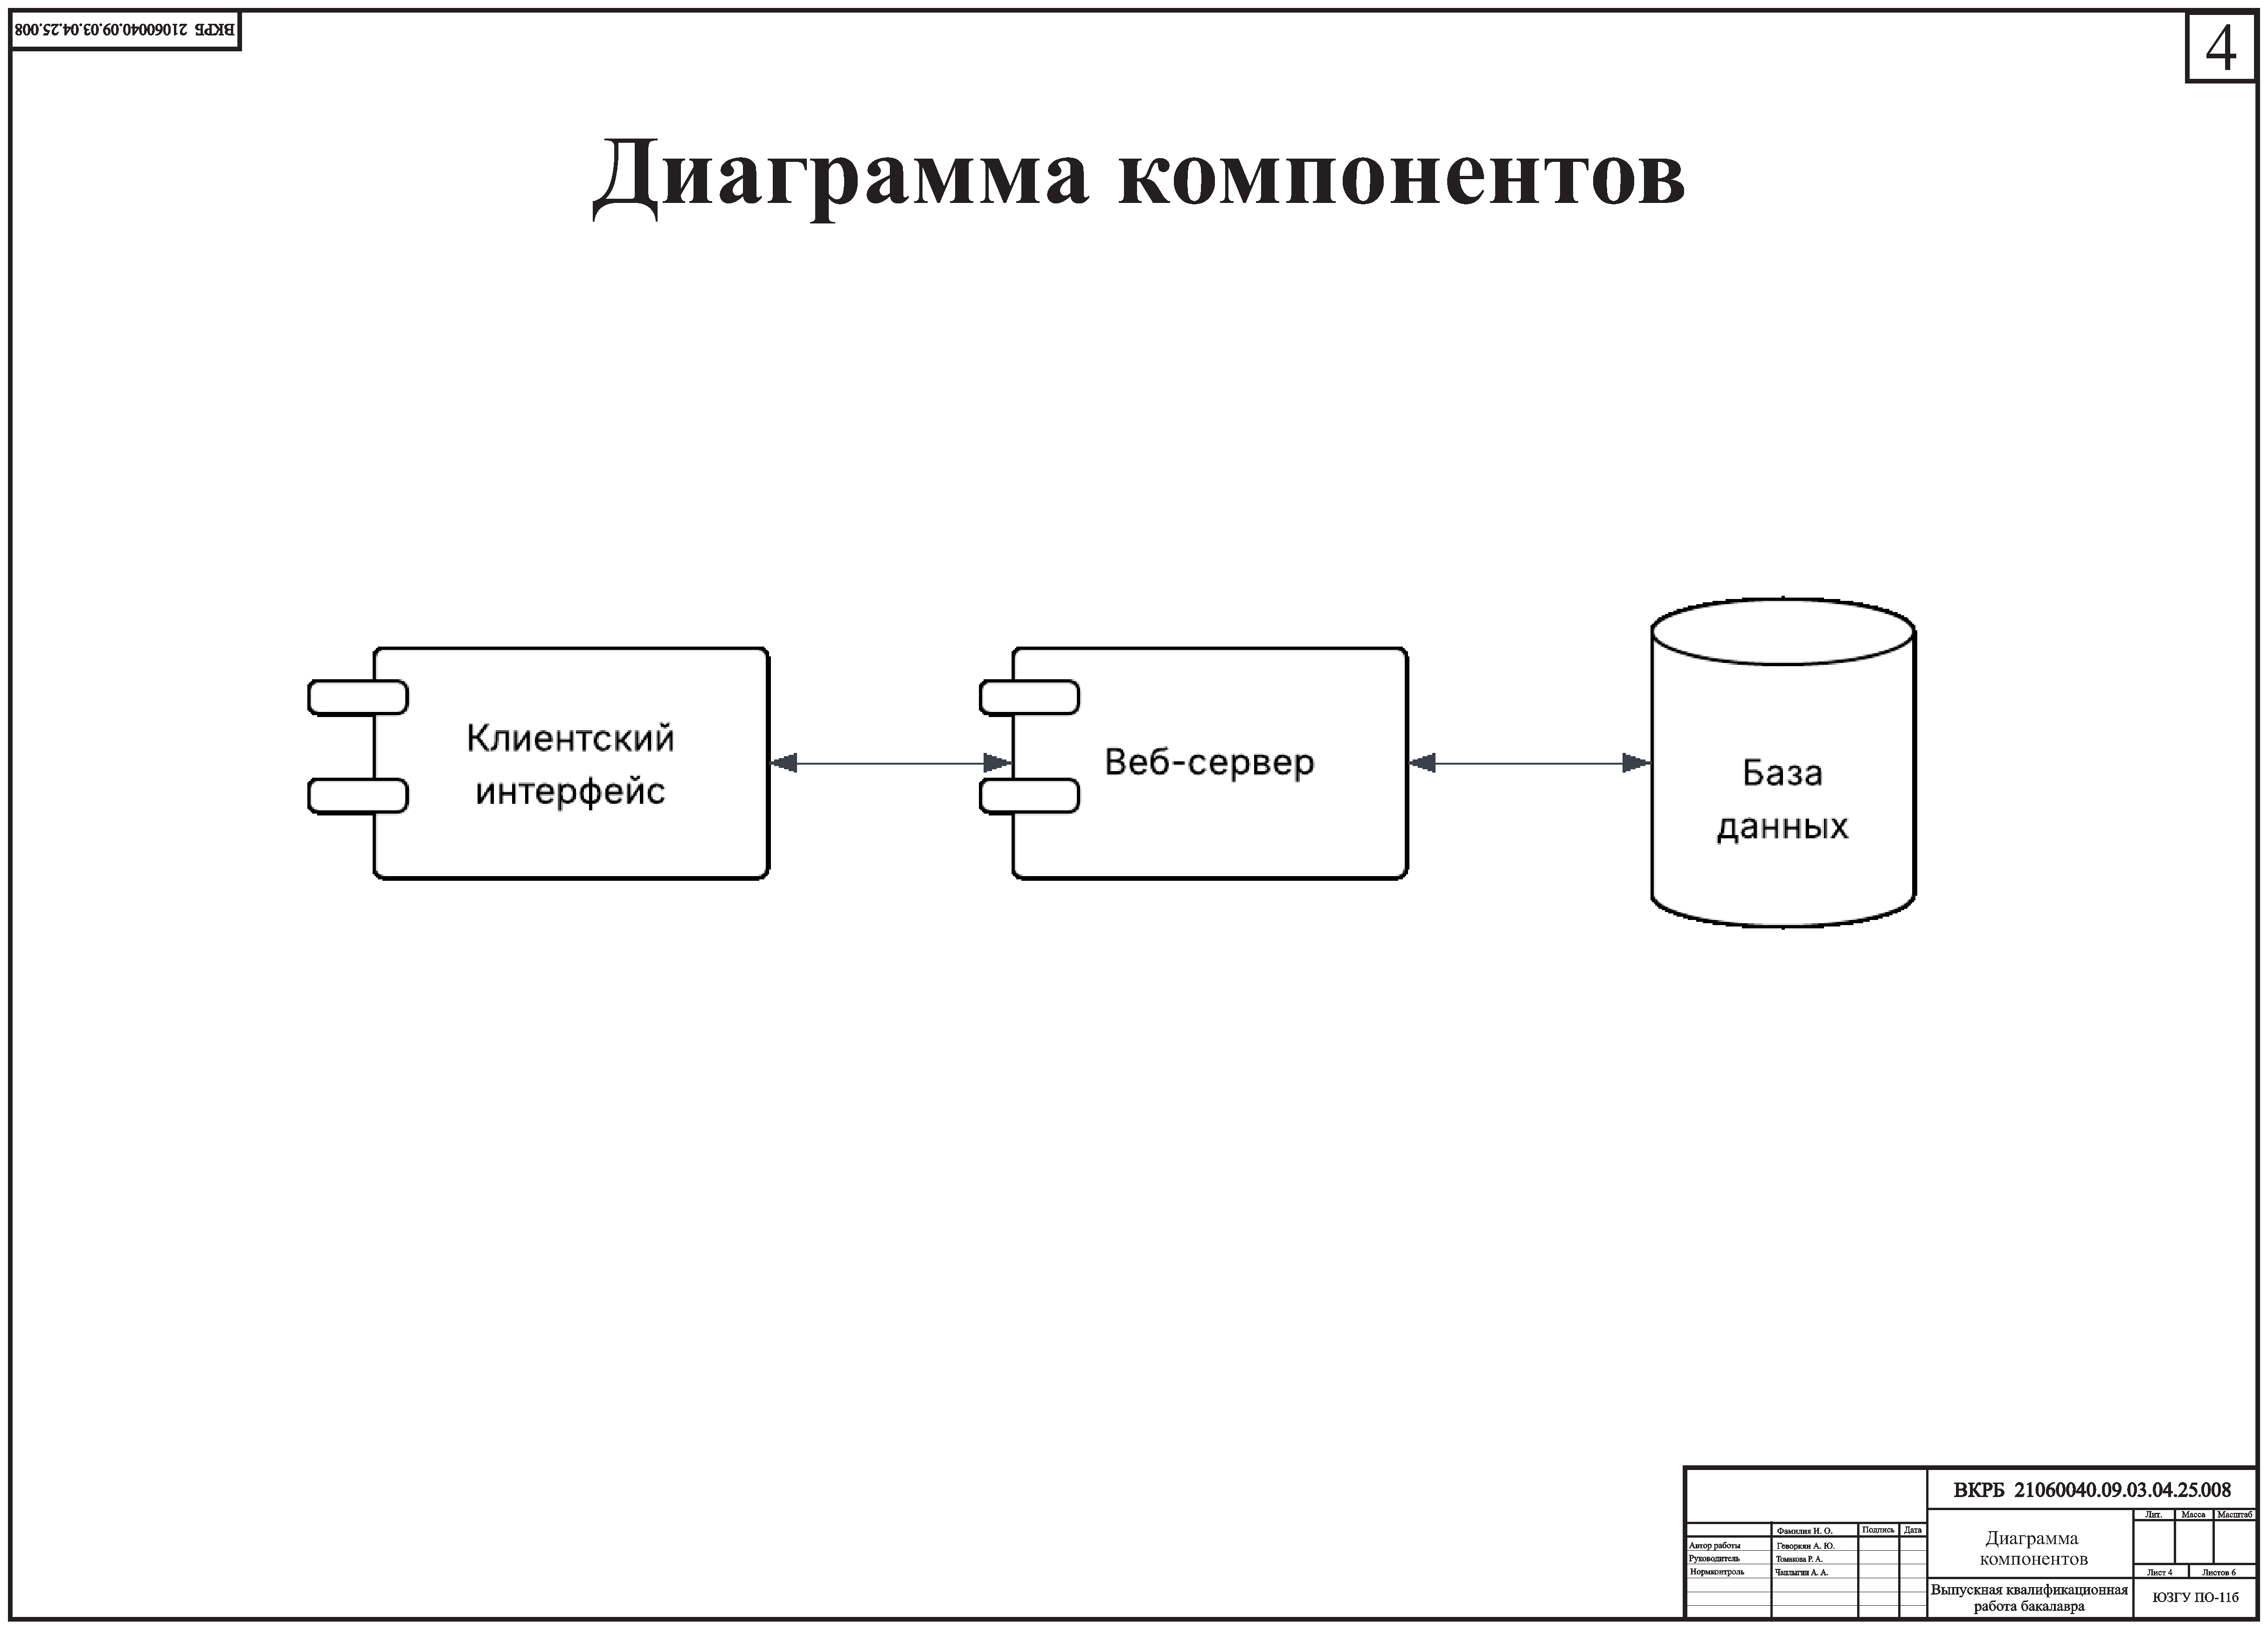
\includegraphics[width=0.82\linewidth]{плакатКомпоненты.eps}
	\заголовок{Диаграмма компонентов}
	\label{pl4:плакатКомпоненты}      
\end{плакат}

\begin{плакат}
	
\includegraphics[width=0.82\linewidth]{плакатER.eps}
	\заголовок{ER -- диаграмма}
	\label{pl5:плакатER}      
\end{плакат}

\begin{плакат}
	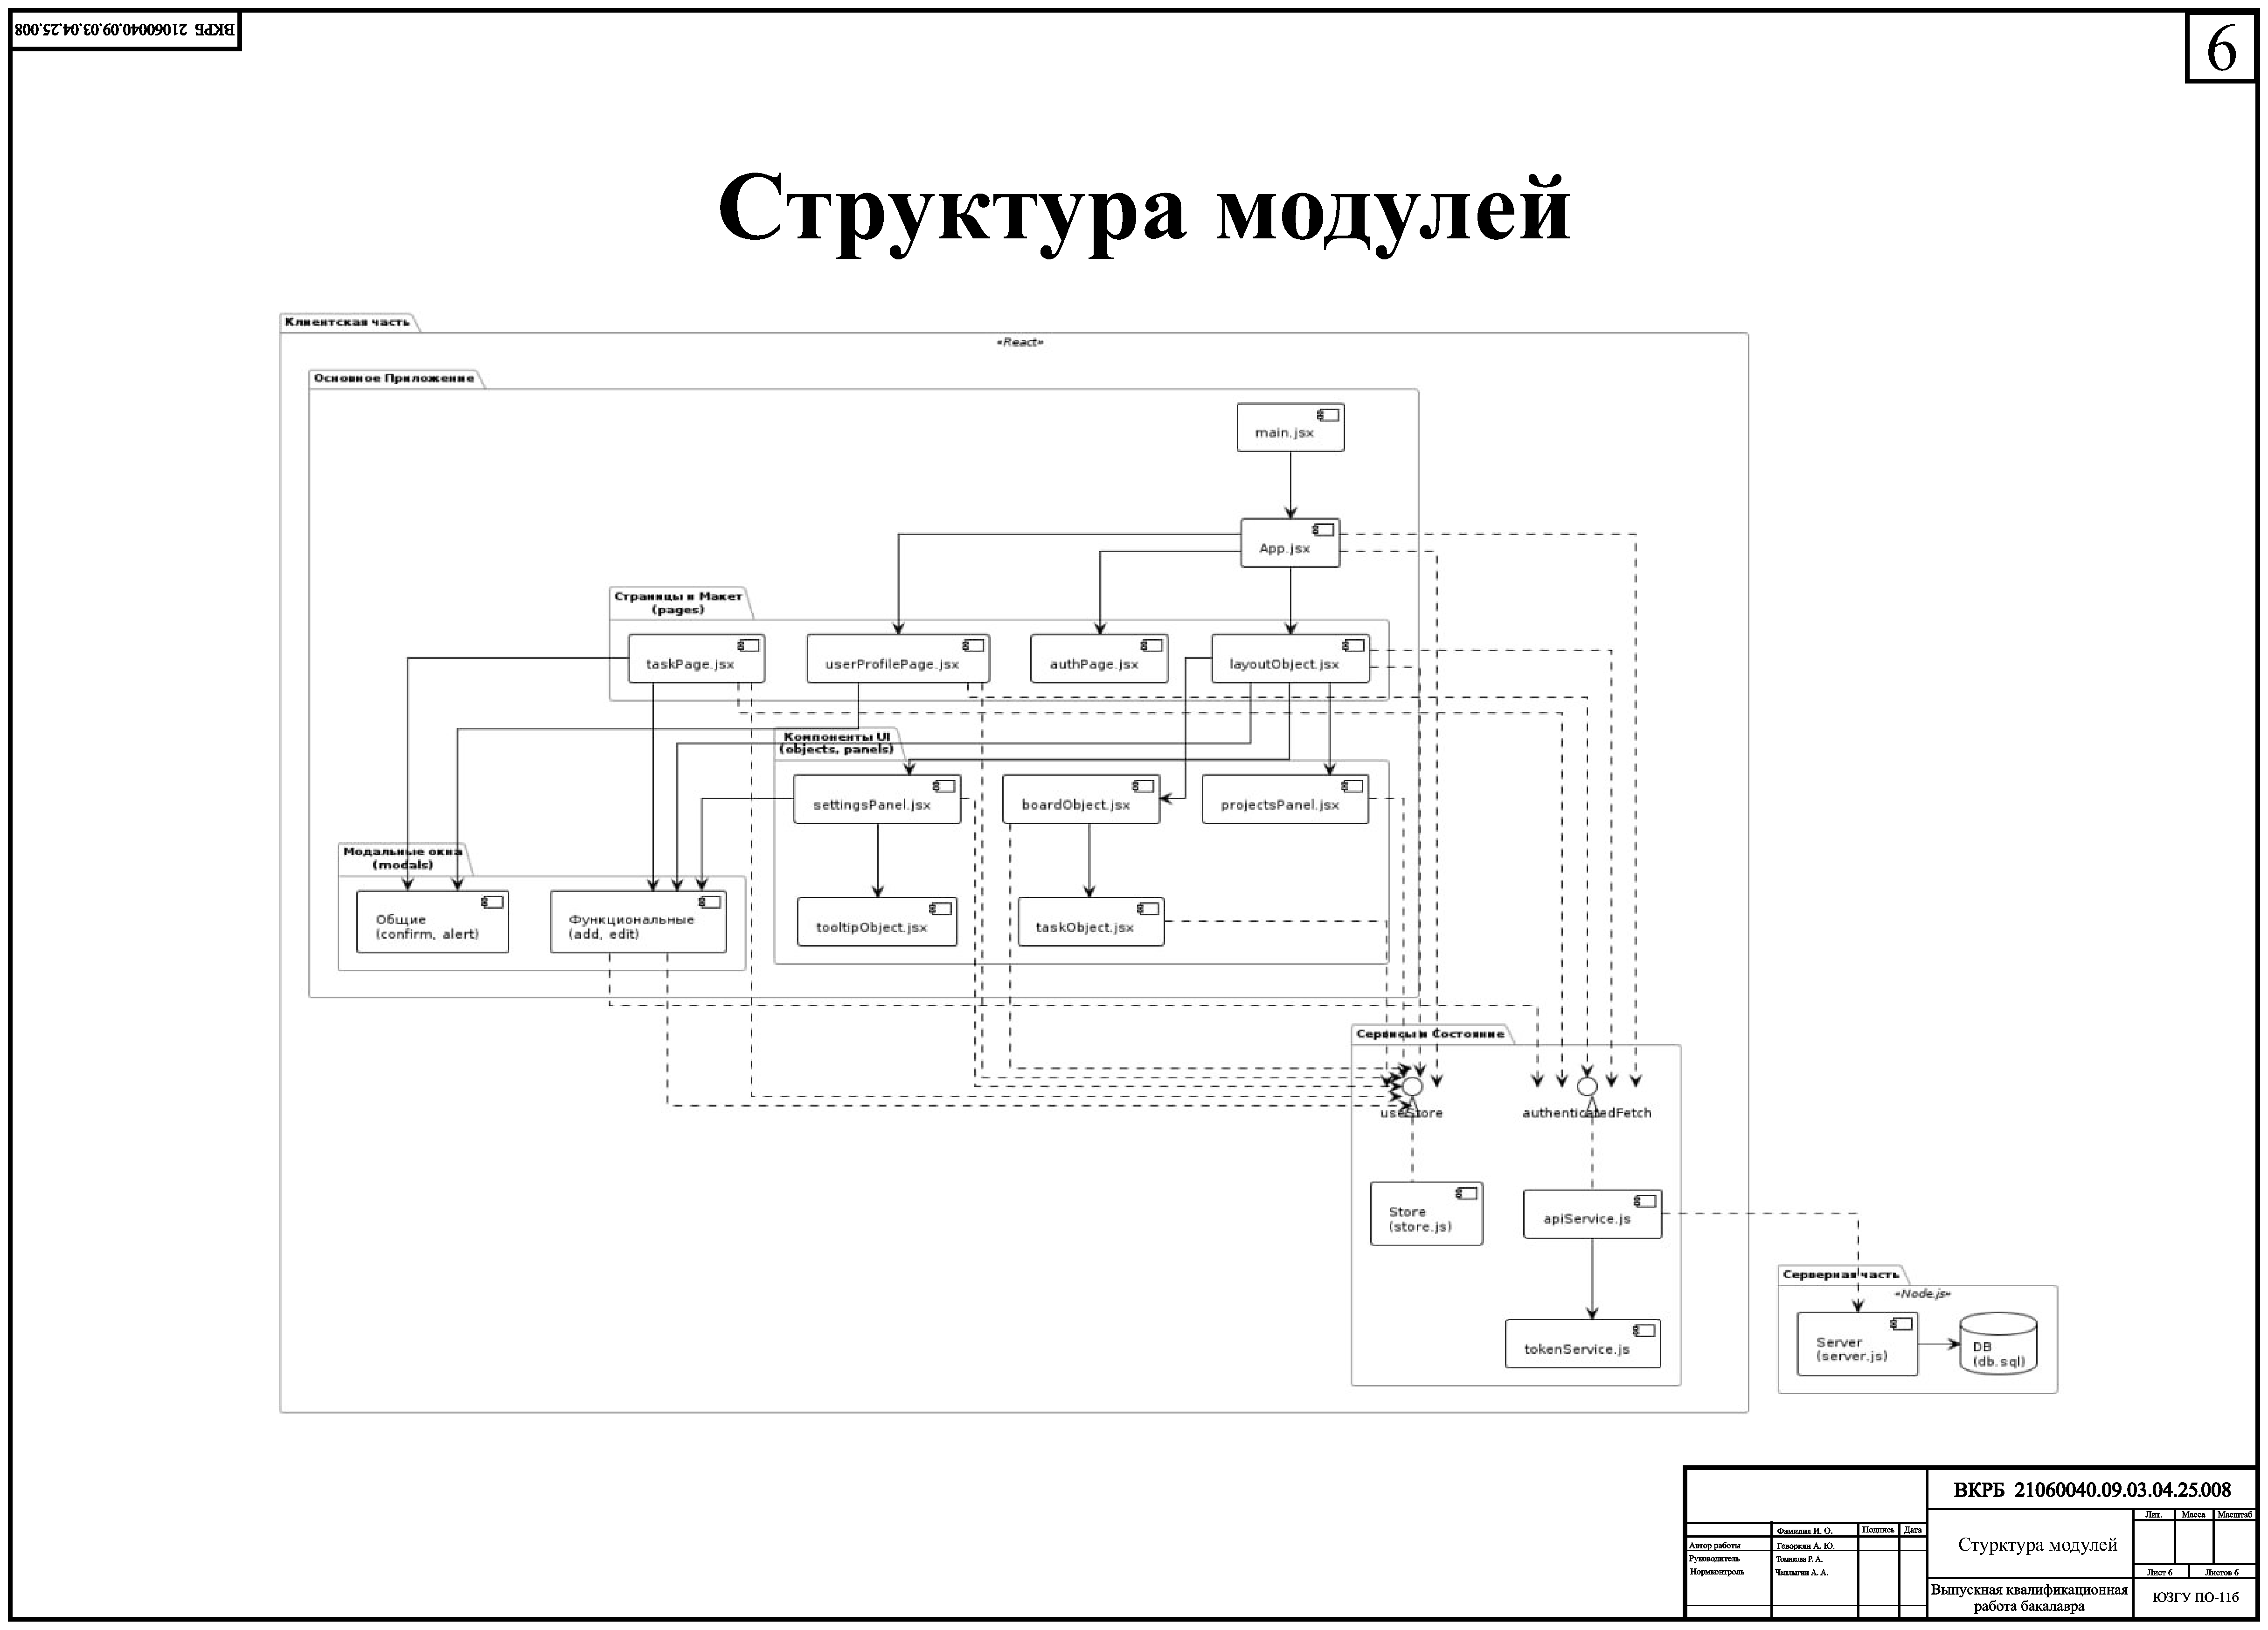
\includegraphics[width=0.82\linewidth]{плакатМодули.eps}
	\заголовок{Структура модулей}
	\label{pl6:плакатМодули}      
\end{плакат}

\begin{плакат}
	\includegraphics[width=0.82\linewidth]{плакатИнтерфейс.eps}
	\заголовок{Результат использования веб-приложения}
	\label{pl7:плакатИнтерфейс}      
\end{плакат}

\begin{плакат}
	
\includegraphics[width=0.82\linewidth]{плакатЗаключение.eps}
	\заголовок{Заключение}
	\label{pl7:плакатЗаключение}      
\end{плакат}

\end{landscape}
